\section{tuberia-bidireccional.c y tuberia-bidireccional-modificado.c}

	Muestre la pantalla de compilación y ejecución de los dos programas.

	\begin{center}
		Centrar la imagen para el primer programa aquí
		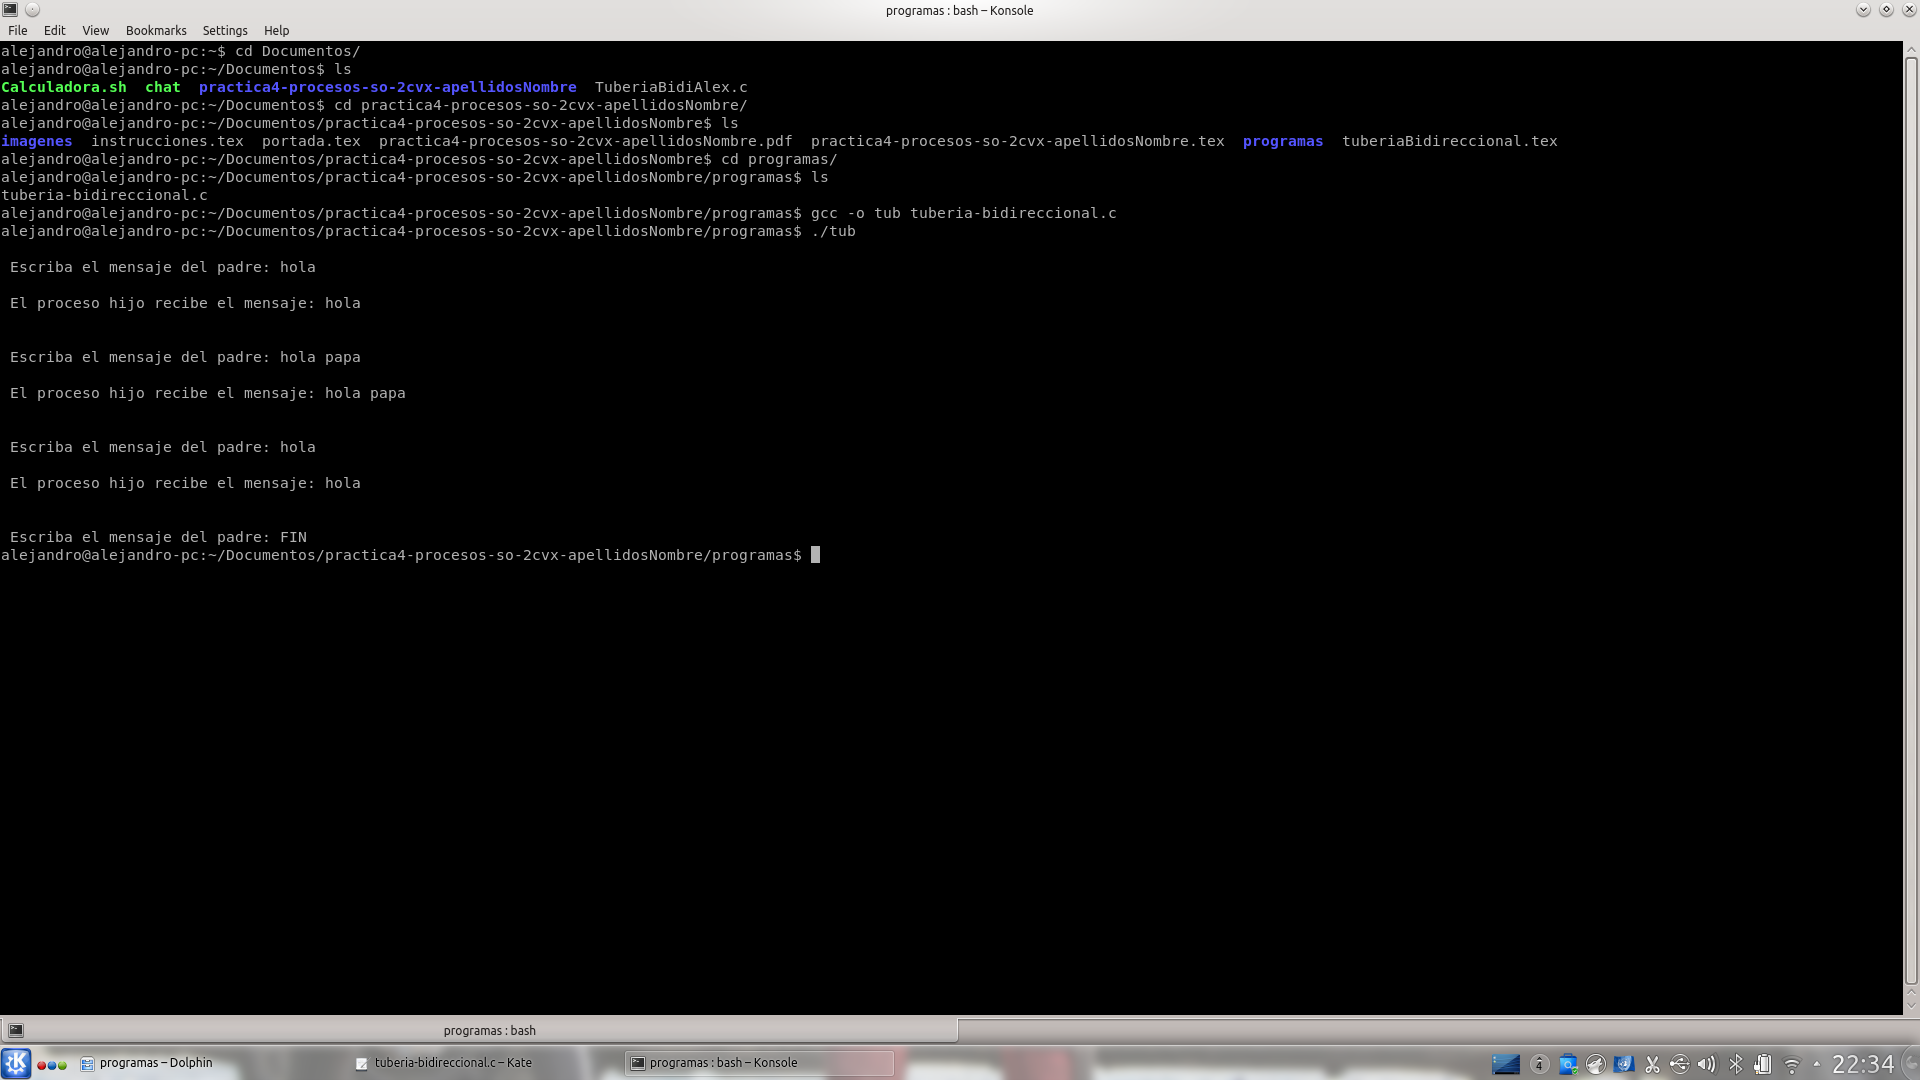
\includegraphics[scale=0.15]{imagenes/1.png}
	\end{center}
	En este programa se utiliza la función pipe() la cual abre una "tubería" de comunicación y nos devuelve dos descriptores de fichero abiertos, uno por cada extremo de la tubería. Esto se trabaja mediante un arreglo de 2 elementos. Por el primero de ellos se puede leer (con read()) lo que se escriba por el segundo (con write()). La ventaja de este mecanismo, es que si creamos la tubería antes de crear el proceso hijo (antes de llamar a fork()), como el proceso hijo se hace copia de todo lo del padre, también copia la tubería. 
		Tenemos una tuberia bidireccional, al padre le mandan un mensaje y este mismo mensaje es el que recibe el hijo, solo que el hijo no interactua con el padre, solo cumple la función de recibir lo del padre.

	\begin{center}
		Centrar la imagen para el segundo programa aquí
		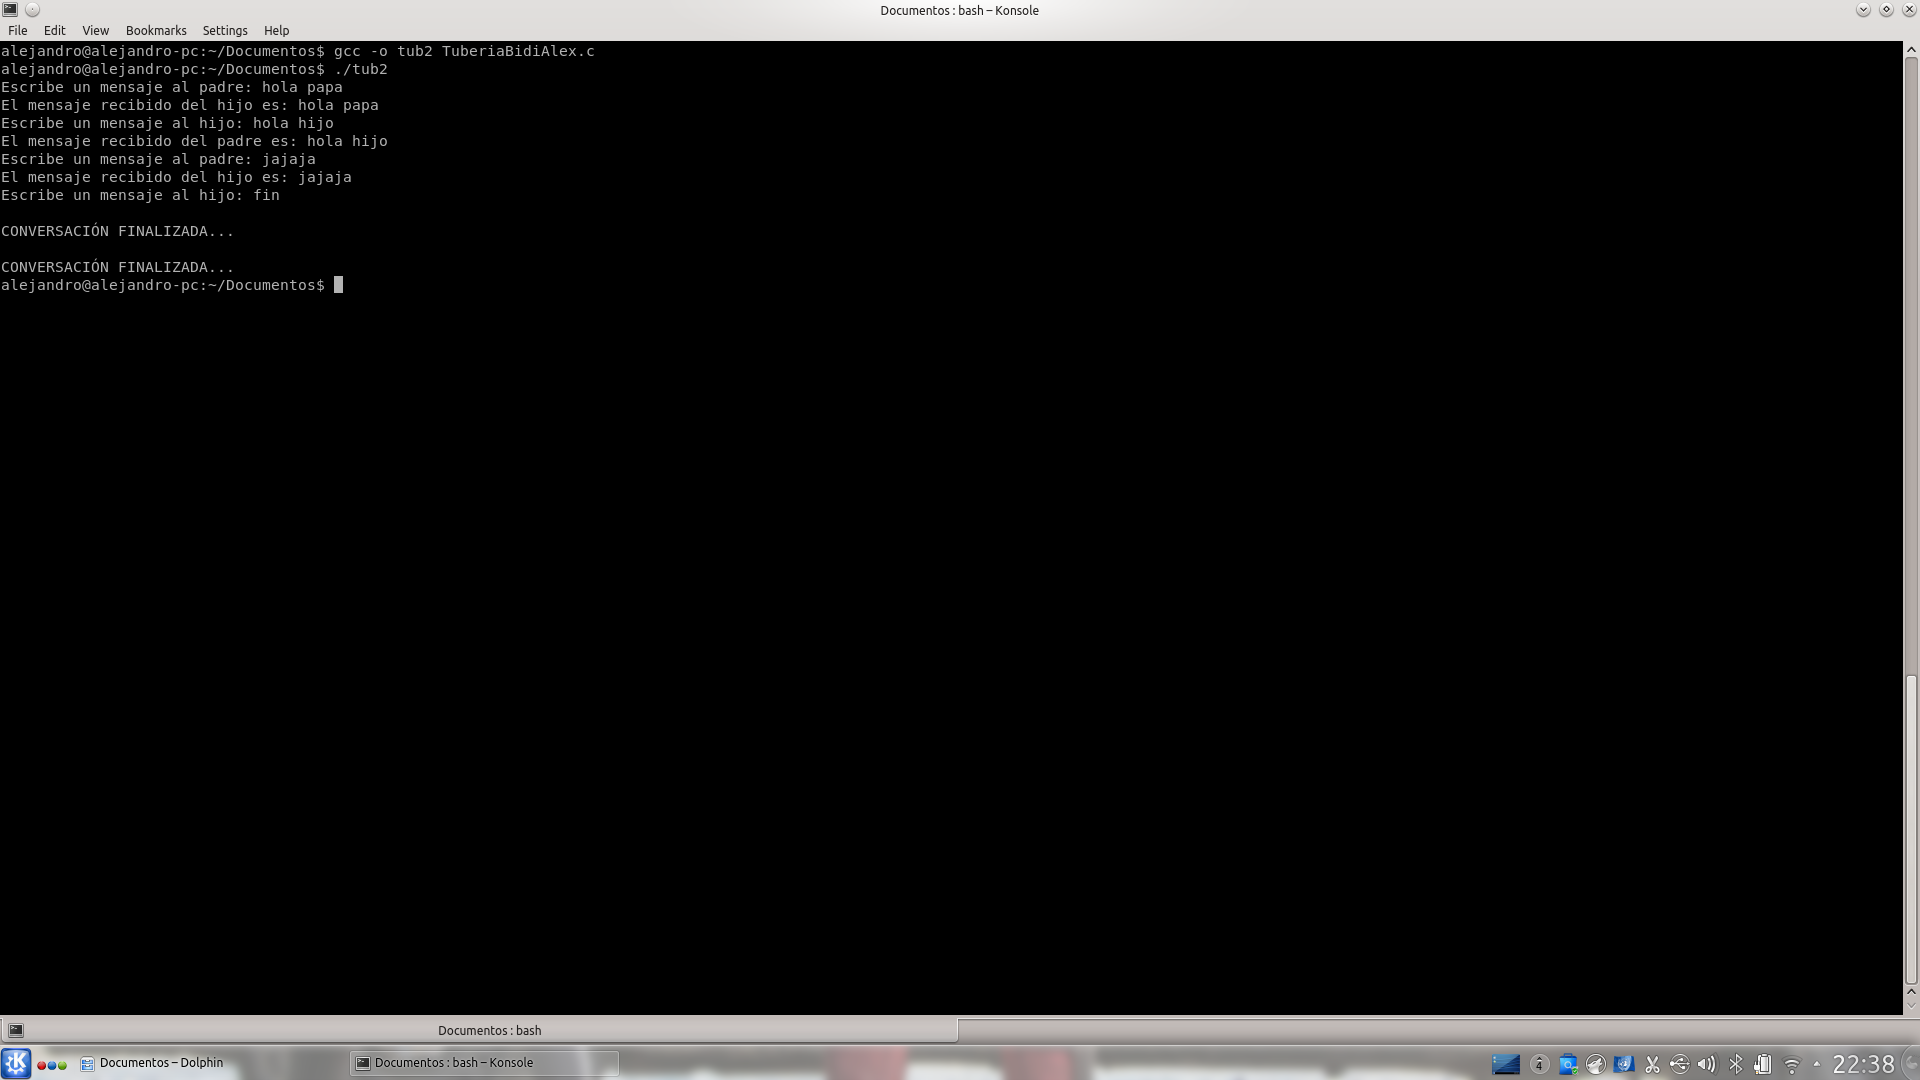
\includegraphics[scale=0.15]{imagenes/2.png}
	\end{center}
	
	En este otro programa ya modificado, el padre recibe mensaje del usuario, este mensaje del padre se le manda al hijo, y el hijo ya interactua con el padre y se puede entablar una "conversación" hasta que el padre manda el FIN de esta conversación, el programa termina. Para realizar el programa se necesita dominar el concepto de "pipe()" ya que se maneja una tubería bidireccional.